\documentclass[a4paper,11pt,ja=standard,lualatex]{bxjsarticle}
\geometry{margin=18mm}
\usepackage{luatexja}
\usepackage{luatexja-fontspec}
\setmainfont{Times New Roman}
\setsansfont{Helvetica}
\usepackage{xcolor}
\usepackage{graphicx}
\usepackage{hyperref}
\usepackage{array}
\usepackage{tabularx}
\usepackage{enumitem}
\usepackage{float}
\usepackage{listings}
\usepackage{tikz}
\usepackage{fancyhdr}
\usepackage{titlesec}
\usepackage{setspace}
\hypersetup{
  colorlinks=true,
  linkcolor=blue!50!black,
  urlcolor=blue!50!black
}

\pagestyle{fancy}
\setlength{\headheight}{18pt}
\fancyhf{}
\lhead{AIレポート}
\rhead{Antigravity + Tetris Project}
\cfoot{\thepage}

\titleformat{\section}{\large\bfseries}{\thesection.}{0.5em}{}
\titleformat{\subsection}{\normalsize\bfseries}{\thesubsection.}{0.5em}{}

\definecolor{codebg}{RGB}{248,248,248}
\definecolor{codeframe}{RGB}{220,220,220}
\definecolor{darkblue}{RGB}{20,60,120}
\definecolor{cyanblock}{RGB}{80,227,230}
\definecolor{blueblock}{RGB}{36,95,223}
\definecolor{orangeblock}{RGB}{223,173,36}
\definecolor{yellowblock}{RGB}{223,217,36}
\definecolor{greenblock}{RGB}{48,211,56}
\definecolor{purpleblock}{RGB}{132,61,198}
\definecolor{redblock}{RGB}{227,78,78}

\lstdefinestyle{tsstyle}{
  basicstyle=\ttfamily\footnotesize,
  keywordstyle=\color{darkblue}\bfseries,
  commentstyle=\color{gray},
  stringstyle=\color{green!40!black},
  backgroundcolor=\color{codebg},
  frame=single,
  rulecolor=\color{codeframe},
  breaklines=true,
  showstringspaces=false,
  columns=fullflexible
}

\setstretch{1.08}

\begin{document}

\begin{center}
  {\LARGE \textbf{AI技術レポート：Antigravityを用いたTetrisプロジェクトの実行と分析}}\\[4pt]
  {\large 使用したAIサービス：Antigravity}\\[8pt]
  {\normalsize 提出用ドラフト}
\end{center}

\section{（1）やったこと・動かしたものの概要}
本レポートでは、AIコーディング支援サービスである \textbf{Antigravity} を用いて\textbf{Tetris} を\textbf{vibecoding}し、その過程を整理した。対象となるプログラムは React、TypeScript、Vite を用いて作られたブラウザ版での Tetris である。

今回の目的は、\textbf{Antigravity を用いてVibecodingを行い、その有用性と限界を確認すること}である。具体的には、次の作業を行った。

\begin{itemize}[leftmargin=5mm]
  \item AntigravityにTetrisを生成する指示を与える
  \item 生成されたゲームに対して、微調整を行う
  \item 以上の過程を、複数回繰り返しデバグや追加機能を入れた。
\end{itemize}

最終的には以下の機能まで実装が行えた。 

\begin{itemize}[leftmargin=5mm]
  \item テトリミノの落下
  \item 左右移動
  \item 回転
  \item ライン消去
  \item スコア、行数、レベルの更新
  \item Hold 機能
  \item キーによるミノの変更(チートmode)
\end{itemize}

\begin{figure}[H]
\centering
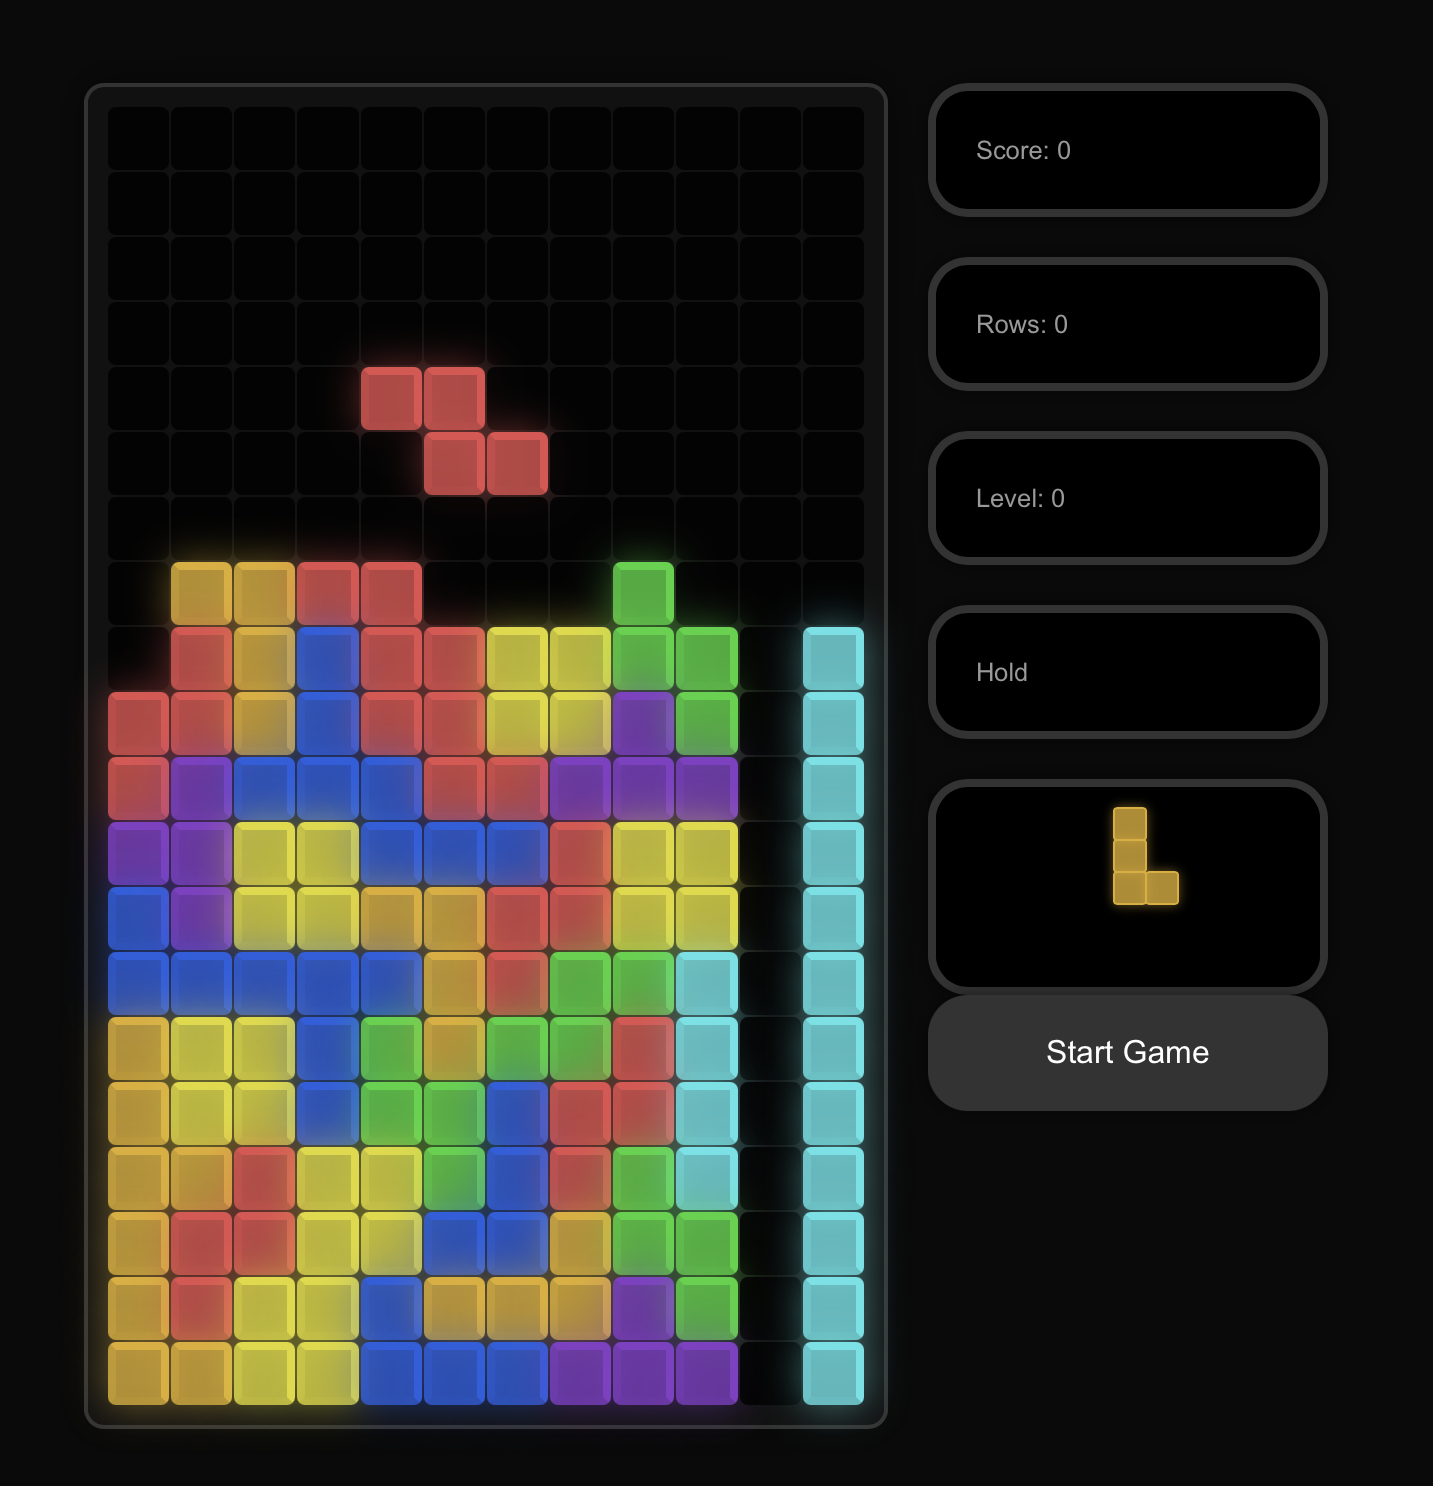
\includegraphics[width=0.7\linewidth]{image2.png}
\caption{作成したテトリスの画像}
\end{figure}

\begin{figure}[H]
\centering
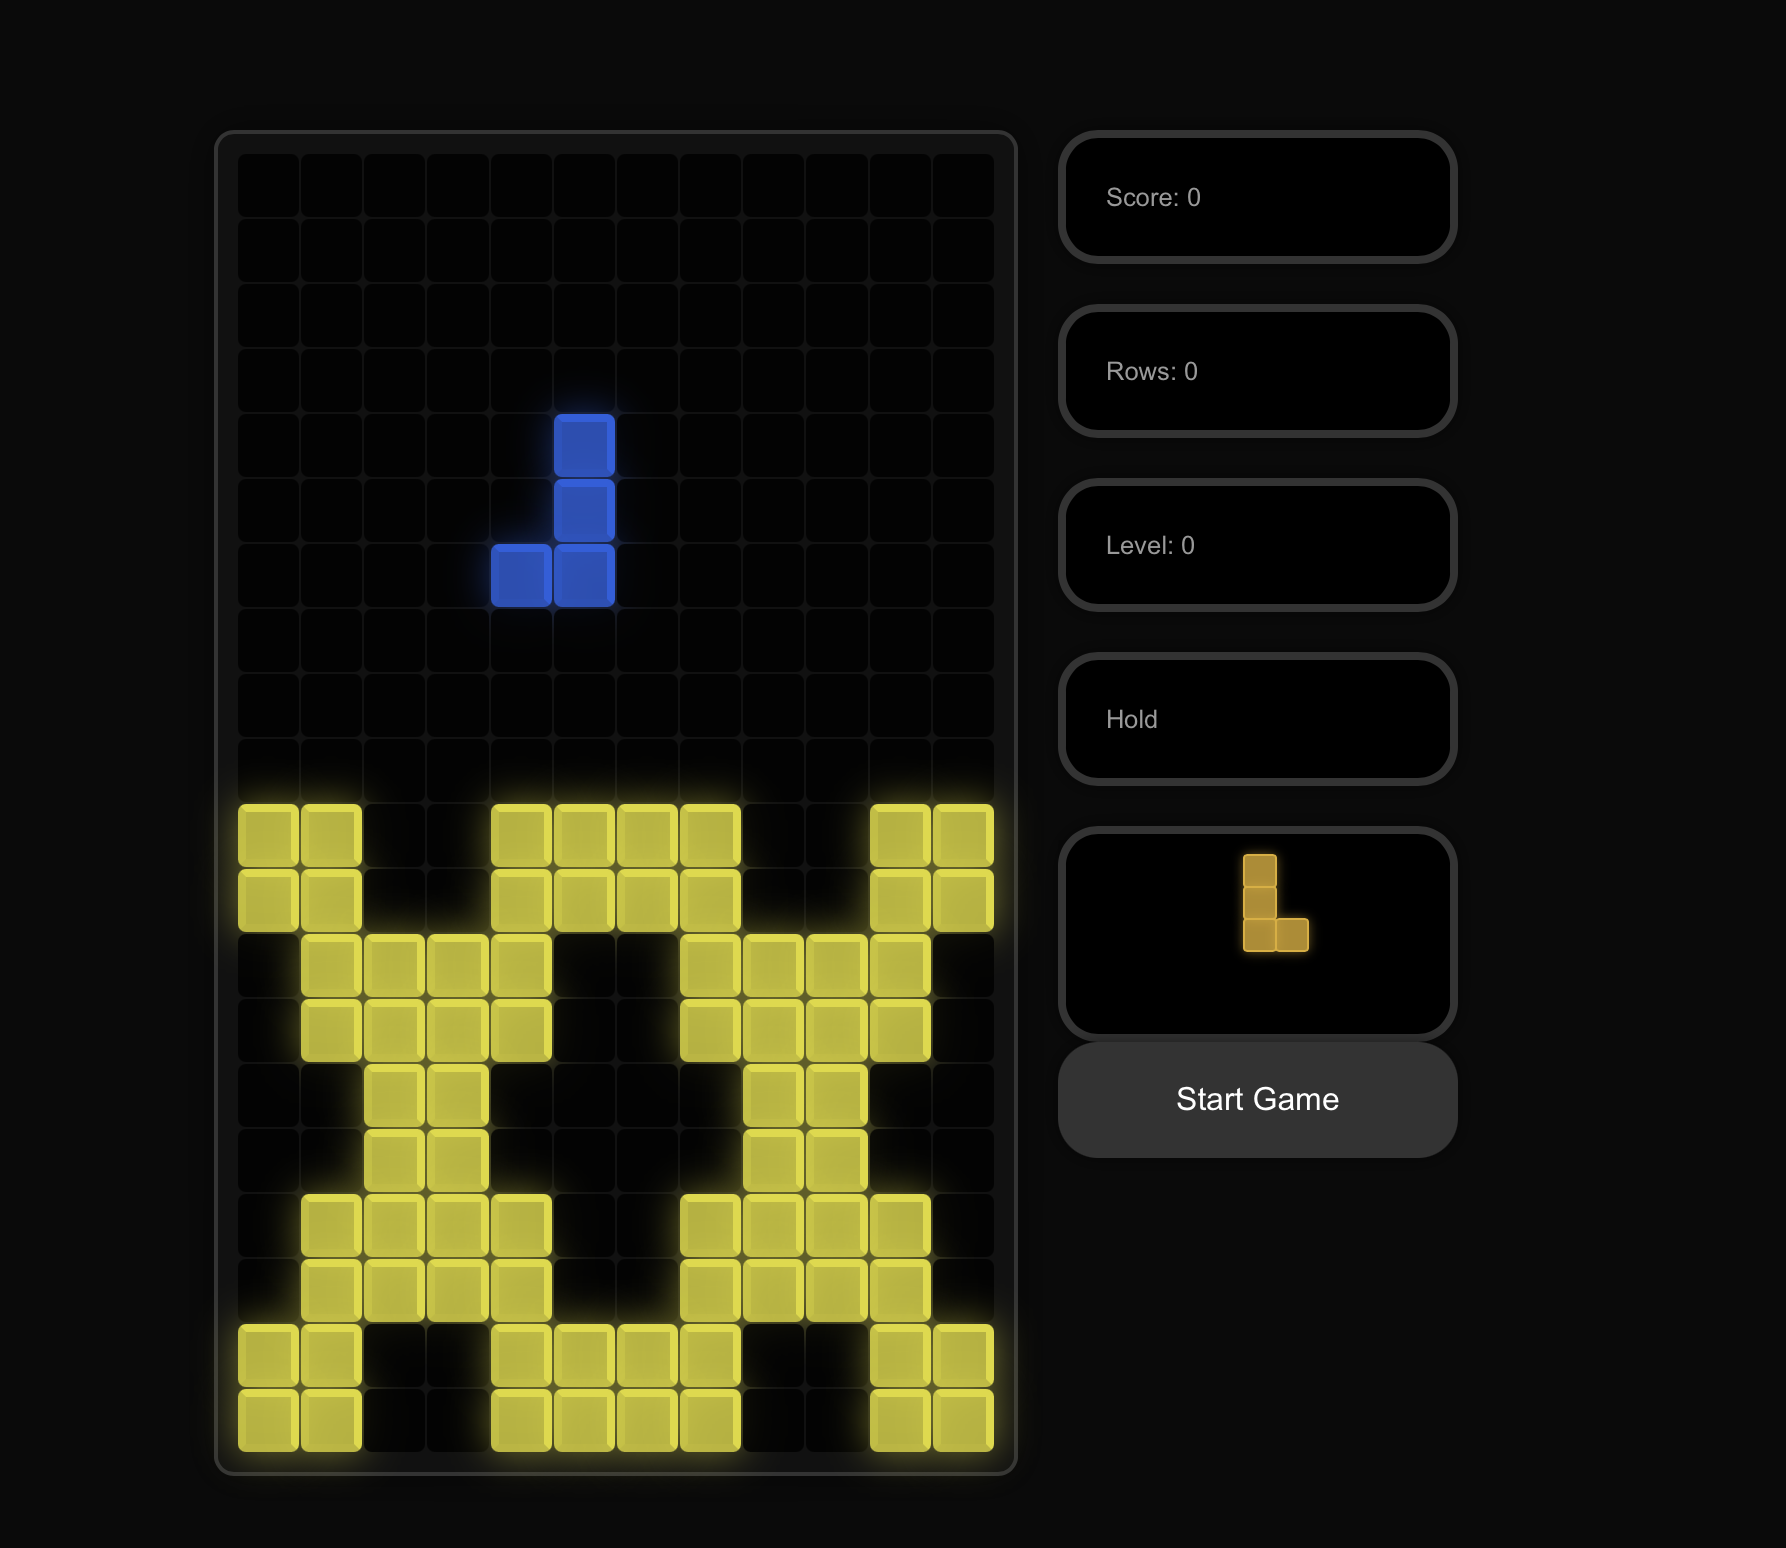
\includegraphics[width=0.7\linewidth]{image.png}
\caption{テトリスですべてoミノにして不正した画像}
\end{figure}

\section{（2）具体的な手続き}
\subsection{実行手順}
実際に行った手順は以下の通りである。

\begin{enumerate}[leftmargin=6mm]
  \item プロジェクトディレクトリを作成
  \item Antigravityの起動
  \item 自然言語のみで、Antigravity　にTetrisを生成するよう伝える(1)
  \item 複数回デバグを行う
  \item 追加機能としてキー入力で任意のミノに変更できるようにした
\end{enumerate}


\subsection{主なデバグ内容}
\begin{enumerate}[leftmargin=6mm]
  \item 一番最初の指示で綺麗に生成することはできなかった。
  \item 主な原因は左右の壁に当たるとその場で止まってしまう。
  \item 左右の壁が繋がってしまい、左右が通り抜けることができる。
\end{enumerate}

\section{（3）評価・考察}

\subsection{Antigravityのメリット}
\begin{enumerate}[leftmargin=6mm]
  \item 知らない言語に対して、実行したいものを瞬時に作成ができる。
  \item １時間程度でゲームが作成できたため、最低限のコードエージェントとして活用できる。
  \item デバグしてほしい内容に対して適切にデバグできた。
\end{enumerate}

\subsection{Antigravityのデメリット}
\begin{enumerate}[leftmargin=6mm]
  \item 内部の構成がわからないため、セキュリティなどには不安が残る
  \item 最初から完璧に作ることはできなかった
  \item デバグの量もかなりあった。
\end{enumerate}

\subsection{今後の検証候補}
\begin{enumerate}[leftmargin=6mm]
  \item より高度な検証をするため、より複雑なゲームの生成を試みる。
  \item 同じゲームをcodex やclaudeにも書かせることでモデルやAgentの比較を行う
  \item プロンプトの設定による性能の変化を検証する。
\end{enumerate}


\section{まとめ}
本レポートでは、AI 技術として \textbf{Antigravity} を用い、その実行後に得られた React + TypeScript 製の Tetris プロジェクトを生成した。

その結果、Antigravity のようなAIコーディング支援は、短時間でアプリケーションの土台を得る手段として有用である一方、生成結果をそのまま提出できるとは限らず、\textbf{人間が実行して確認し、必要な修正を加えることが不可欠である}と分かった。

今回の体験を通じて、AI は「完全自動で完成品を出すもの」というより、\textbf{開発の初速を上げる補助ツール}として使うのが現実的であると感じた。


\vfill
\noindent\textbf{付録：提出確認に用いたコマンド}\\
\texttt{npm run build}

\end{document}
